\section{Kalman Filters}
Traditionally, the Kalman Filter (KF) is a tool used to analyse a set of linear data points for an unknown dynamic model. Each data point is passed in 1-by-1 to the filter (thus the k$^{th}$ step involves the k$^{th}$ data point) using the following nomenclature:\newline

$\hat{x}_{k|k}$ [nx1]:    the k$^{th}$ estimated state space given the first k observations ($z_{1} \cdots z_{k}$)\newline
$\hat{x}_{k+1|k}$ [nx1]:  the k+1$^{st}$ estimated state space given the first k observations ($z_{1} \cdots z_{k}$)\newline
$F_{k}$ [nxn]:  the state transition function\newline
$B_{k}$ = the control input model \newline
$U_{k}$ = the input conrol vector\newline
$P_{k|k}$ [nxn]:  the error covariance matrix (the confidence in) $x_{k|k}$\newline
Q [nxn]:    the processing noise (confidence in the predictions)\newline
$H_{k}$ [1xn]: the observation model at step k\newline
$z_{k}$ [1x1]: the observation at step k\newline
$y_{k}$ [1x1]: the estimate residual at step k\newline
R [1x1]: the measurement noise (confidence in the obervations)\newline
$S_{k}$ [1x1]: the innovation covariance\newline
$K_{k}$ [nx1]: the kalman gain\newline

Assuming a state space with n parameters, each of these is a matrix with dimensions [AxB] meaning it has A rows and B columns. There exists a proper pairing of Q and R for each dataset, however, they are usually not known. They represent artifacts of the Kalman filters' assumptions that the noise in the data is Gaussian (normally distributed) with mean 0 (i.e. white noise). Q is the covariance matrix of a multivariate normal distribution centered at $\mu$
\begin{equation}
    \mu = [\mu_{1}, \cdots , \mu_{n}], \mu_{i} = 0  \forall i
\end{equation}

 where n is the number of elements in the state space $\hat{x}_{k}$. This acts as the assumed known variability in each of the n parameters in $\hat{x}_{k} \forall k$. Larger entries in Q correspond to larger variability in x which implies a lower confidence in the predicted $\hat{x}_{k}$. R is the variance of a univariate normal distribution centered at 0. This acts as the assumed known variability in all observations $z_{k} \forall k$. In effect, this means
 
\begin{subequations}
\begin{align}
    \Delta \hat{x}_{k} \sim \mathcal{N}(\mu,\,Q) \\
    \Delta z_{k} \sim \mathcal{N}(0,R) 
\end{align}
\end{subequations}

Given the appropriate values of Q and R, the KF acts as an optimal estimator as it minimizes the Mean Square Error (MSE) of the predicted x. In practice, this can be thought of as nearly equivalent to a recursive weighted least squares (WLS) estimate where Q acts as the forgetting factor for the KF as lambda does in WLS. 

\subsection{Our Application of the Kalman Filter}
Normally, the Kalman Filter is used to smooth out noise while maintaining the general form of the original data. As seen in Figure 3.1, the KF takes the set of noisy observations and is able to reconstruct a good approximation of the true function's behavior.

\begin{figure}[h]
\centering
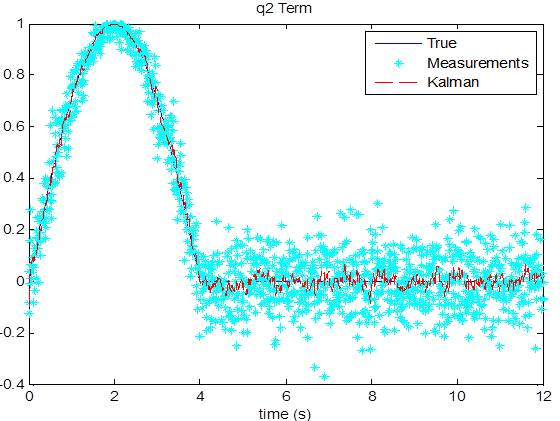
\includegraphics{body/methodology/q2_kalman.jpg}
\caption{Temperary Kalman Filter Picture}
\end{figure}

 For our application, we chose to instead use it to approximate the parameters to a function that best fits the data and from those parameters,then forecast what the value should be at some time in the future. Our implementation is as follows:

We will assume we have some set of noisy linear data in the form (time, value) such that we want to find the best linear approximation of the form 

\begin{equation} 
Value = \hat{B_{0}} + \hat{B_{1}}*time  
\end{equation}

that fits this data. We start with an initial state space estimate of $\hat{x}_{0|0}$, error covariance matrix estimate $P_{0|0}$ and chosen values of Q and R.

\begin{subequations}
\begin{align}
    x_{0|0} &= \begin{bmatrix}
           B_{0} \\
           B_{1}
         \end{bmatrix}
 \end{align}
  \begin{align}
    P_{k} &= \begin{bmatrix}
           P_{B_{0}}&0 \\
           0&P_{B_{1}}
         \end{bmatrix}
  \end{align}
  \begin{align}
    Q &= \begin{bmatrix}
        Q_{B_{0}}&0 \\
        0&Q_{B_{1}}
        \end{bmatrix}
  \end{align}
  \end{subequations}
  
  \subsubsection{KF Prediction}
  
  The first step is prediction. We calculate $x_{k|k-1}$ and $P_{k|k-1}$ at the current iteration based on the last iteration's $x_{k-1|k-1}$ and $P_{k-1|k-1}$.
  
  \begin{subequations}
  \begin{align}
  \hat{x}_{k|k-1} = F_{k} \hat{x}_{k-1|k-1}+B_{k}u_{k}   \\
  P_{k|k-1} = F_{k} P_{k-1|k-1}F_{k}^{T}+Q
  \end{align}
  \end{subequations}
  
  For our purposes, we assumed $F_{k}$ is always identity, meaning our model does not change with time. We also assume $B_{k}u_{k} = 0 \forall k$.
  
  \begin{align}
    F_{k} &= \begin{bmatrix}
           1&0 \\
           0&1
         \end{bmatrix}
         \forall k
  \end{align}
  
  Since any matrix multiplied by identity is always the original matrix, this reduces our prediction equations to the form
  
  \begin{subequations}
  \begin{align}
  \hat{x}_{k+1|k} = \hat{x}_{k|k}   \\
  P_{k+1|k} = P_{k|k}+Q
  \end{align}
  \end{subequations}
  
  This is a simplification as we know the true function is not constant as can be seen from figures 3.2 - 3.4. These changes shift the filter from dynamic to a nearly static static model approximation. P represents the confidence in (or variability of) each parameter in the current state space with larger values of P implying less confidence in $\hat{x}$. From Equ. 3.7b we can see that providing a larger Q causes consistently larger estimates of P. This makes sense as Q is a measure of the variability in each parameter of x, so larger Q's should cause the KF to be less confident in it's predictions.
  
  As a further simplification, we assumed P and Q to be 0 in the off diagonal as shown in Equs. 3.4b and 3.4c. This means we assume that the parameters B$_{0}$ and B$_{1}$ exist and change independently where  P$_{B_{0}}$,  P$_{B_{1}}$, Q$_{B_{0}}$, and Q$_{B_{1}}$ can be any non-negative real numbers.
 
 \subsubsection{KF Updating}
 
  The second step is updating. Each iteration of the KF utilizes a single data point, so the k$^{th}$ iteration will use the point (Time$_{k}$, Value$_{k}$). We begin by calculating the residual (or error from the k$^{th}$ known observation) for (Time$_{k}$, Value$_{k}$).
  
  \begin{equation}
  \centering
  y_{k} = z_{k} - H_{k}\hat{x}_{k|k-1}
  \end{equation}
  
  Here H$_{k}$ is
  
  \begin{align}
    H_{k} &= \begin{bmatrix}
           1&Time_{k}
         \end{bmatrix}
  \end{align}
  
  From Equ. 3.4a, we can see 
  
  \begin{equation}
  \centering
H_{k}\hat{x}_{k|k-1} = B_{0}*1 + B_{1}*Time_{k} = \hat{Value}_{k}
  \end{equation}
  
  Thus, y$_{k}$ is simply the difference between the prediction of Value$_{k}$ at Time$_{k}$ and the actual observed Value$_{k}$ at Time$_{k}$.
  
  We then perform the innovation step where we calculate S$_{k}$. S$_{k}$ can be understood as a metric for the confidence in observation z$_{k}$ as it represents the variability of z$_{1}$, \cdots , z$_{k}$. If the values of z$_{1 \cdots k}$ tend to vary greatly, S$_{k}$ will be large. If the values of z$_{1 \cdots k}$ only vary slightly, S$_{k}$ will be small. Larger values of R also cause larger values of S$_{k}$ as seen in Equ. 3.11 since R is a measure of the variability for all observations.
  
  \begin{equation}
  \centering
s_{k} = R + H_{k}P_{k|k-1}H_{k}^{T}
  \end{equation}
  
  P, H, and s come together to form K$_{k}$, the Kalman gain. Kalman gain can be thought of as a ``velocity factor'' of sorts for the KF controlling the magnitude of adjustment to make to the current x$_{k}$. The formula for the optimal gain, meaning it minimizes the mean square error of the estimate, is  
  
    \begin{equation}
  \centering
K_{k} = P_{k|k-1}H_{k}^{T}s_{k}^{-1}
  \end{equation}
  
  From this we can see that as P$_{k}$ gets small, so too does K$_{k}$. This is because a small P$_{k}$ implies high confidence (or low variability) in x$_{k}$. Thus, having high confidence in the current state should yield only a small change to the new predicted x$_{k}$. We can also see that as s$_{k}$ gets large, K$_{k}$ gets small. This also makes sense since large s$_{k}$ implies low observation confidence (or high observation variability). In that case we'd want a smaller state adjustment for larger prediction errors as we don't trust the  current observation as true (that is we want our state adjustment to be less sensitive to erroneous predictions).
  
  We then improve the current state space estimate using information from the k$^{th}$ iteration thus transitioning from $\hat{x}_{k|k-1}$ to $\hat{x}_{k|k}$
  
  \begin{subequations}
  \begin{align}
    \Delta\hat{x}_{k} = K_{k}y_{k} \\
    \hat{x}_{k|k} = \hat{x}_{k|k-1} + \Delta\hat{x}_{k}
    \end{align}
   \end{subequations}

From Equ. 3.13a we see that $y_{k}$ controls the sign of the state prediction adjustment. When z$_{k} < H_{k}\hat{x}_{k|k-1}, y_{k} < 0$ making $\Delta\hat{x}_{k}$ negative. This means if $\hat{x}_{k|k-1}$ over/under estimates $z_k$, the new $\hat{x}_{k|k}$ will be smaller/larger respectively in response. We can also see that the magnitudes of y$_{k}$ and K$_{k}$ control the magnitude of $\Delta\hat{x}_{k}$.

We perform the same improvement for P, changing P$_{k|k-1}$ to P$_{k|k}$ by

\begin{equation} 
\centering
P_{k|k} = (I - K_{k}H_{k})P_{k|k-1}(I - K_{k}H_{k})^{T} + K_{k}RK_{k}^{T}
\end{equation}

where I is the 2-by-2 identity matrix. When using the optimal Kalman gain, as we do, this calculation can be reduced to 

\begin{equation} 
\centering
P_{k|k} = (I - K_{k}H_{k})P_{k|k-1}
\end{equation}

Each iteration k will use the previous iterations estimates of $\hat{x}_{k-1|k-1}$ and P$_{k-1|k-1}$ as the new starting guess for $\hat{x}$ and P while maintaining the same Q and R throughout. Once completed for all data points, the final $\hat{x}_{k|k}$ is treated as the model prediction. We can then use those values of $\hat{B}_{0}$ and $\hat{B}_{1}$ to forecast what the value will be for some time in the future. Since the KF processing data point by point, data can be fed in in any order with the forgetting factor Q weighting the later processed points more heavily. Our time series data comes in chronological order, so Q allows us to essentially weight the more recent data more heavily. This is effectively equivalent to performing a WLS fit.

Figure 3.2 shows an example of a line whose parameters were found using the KF with an all zero Q along side the same contest fit with a line by ordinary least squares. Both approaches predict virtually the same line. However, if Q is changed such that Q$_{B_{0}}$ = 0.3  instead of 0 as in figure 3.3, we can see the behavior changes significantly.

\begin{figure}[h]
\centering
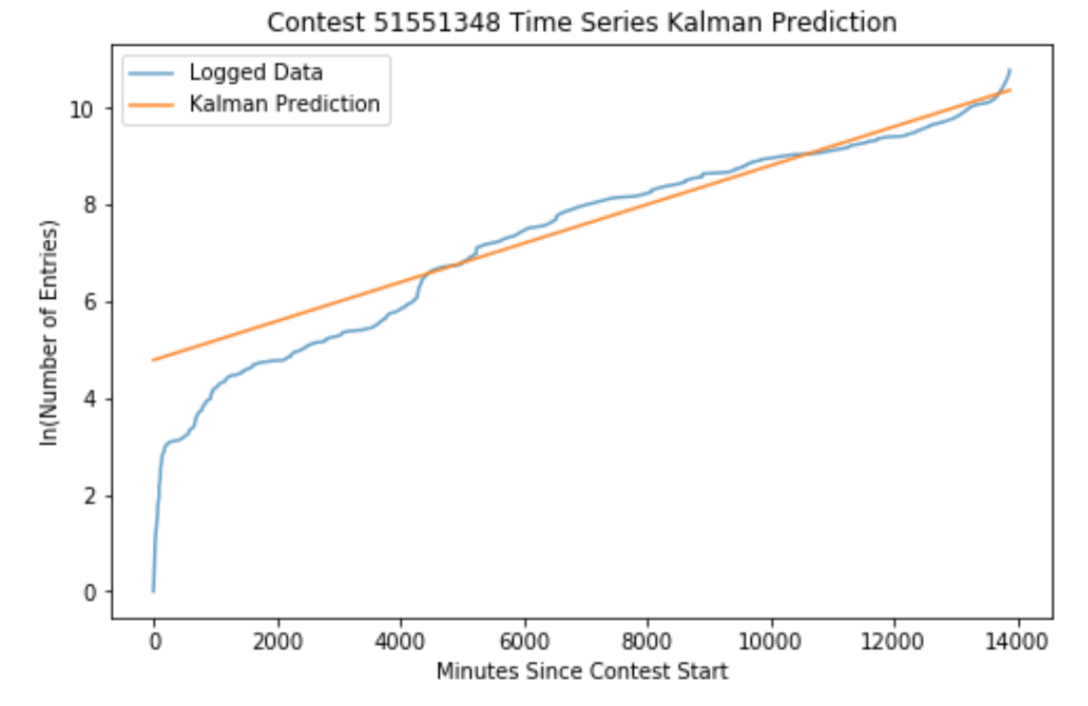
\includegraphics[width=8cm]{body/methodology/KF_Q0.png}
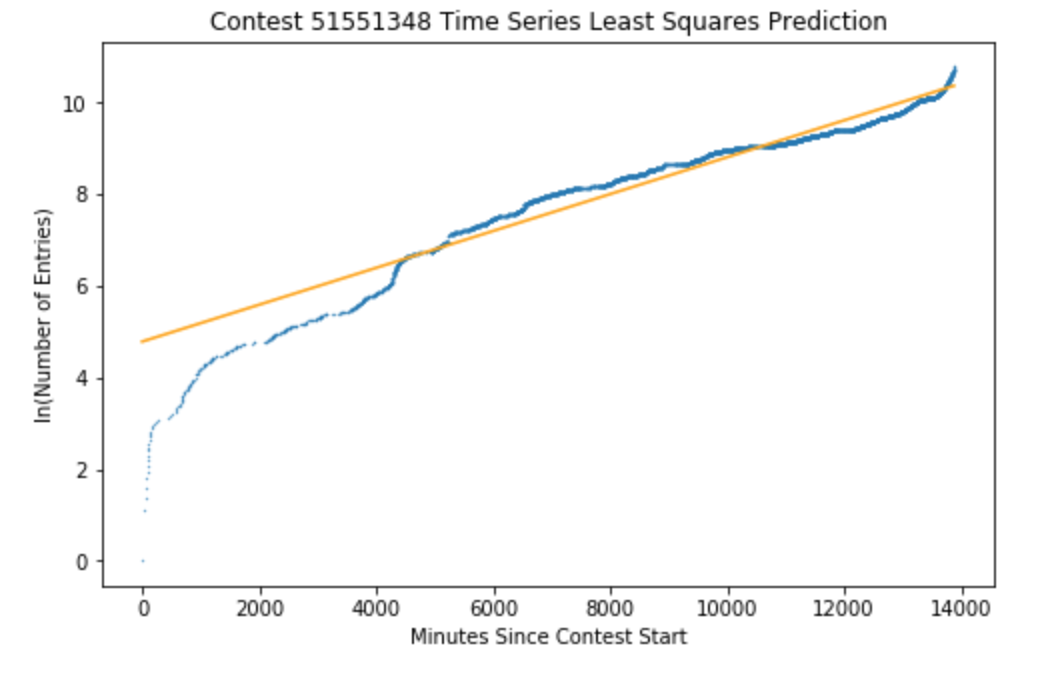
\includegraphics[width=8cm]{body/methodology/LS_pred.png}
\caption{Temp linear KF Q=0/ LS predicitons Lam=1}
\end{figure}

Performing the fit by KF can be convenient for time series data as each iteration involves processing only one data point at a time. And while least squares is not very computationally intensive, it still requires redoing the entire dataset calculation when updating the parameters.

\begin{figure}[h]
\centering
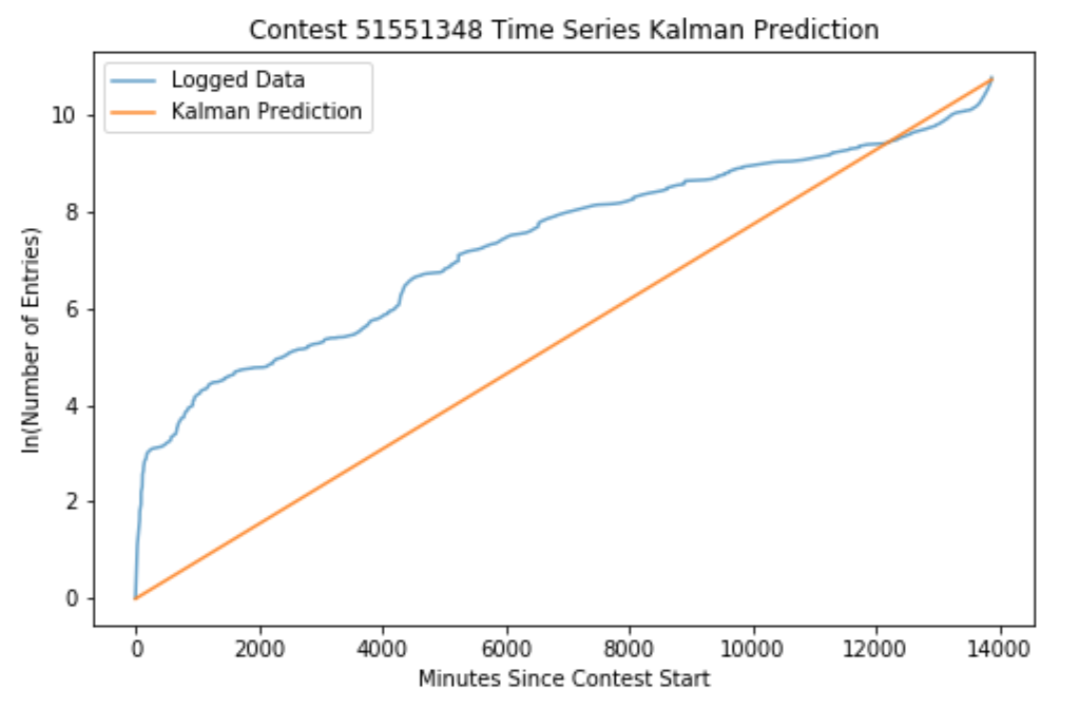
\includegraphics[width=10cm]{body/methodology/KF_Q3.png}
\caption{Temp lin KF Q=0.3}
\end{figure}

\subsection{Extended Kalman Filter}

While the KF is an excellent method for estimating model parameters, it is limited in the same way as LS in that it can only predict for linear models. This will work for estimating on logged data, however, we'd prefer to be able to directly estimate the parameters of the non-linear exponential function $B_{0}e^{B_{1}t}$. To do this, we turn to the Extended Kalman Filter (EKF). The EKF works exactly the same as the normal KF except it can work with non-linear model functions. The only difference between the KF and EKF for our purposes is the values of H$_{k}$. For the EKF, H$_{k}$ takes the form

\begin{equation}
\centering
H_{k} &= \begin{bmatrix}
           {\frac{\partial M(t)}{\partial B_{1}}&\cdots&\frac{\partial M(t)}{\partial B_{i}}
         \end{bmatrix}
\end{equation}

where $B_{0}$ \cdots B$_{i}$ are the values of the state space $\hat{x}$ and M(t) is the non-linear model function. In our case, we assume M(t) = $B_{0}e^{B_{1}t}$, thus

\begin{equation}
\centering
H_{k} &= \begin{bmatrix}
           e^{B_{1}t}&B_{1}B_{0}e^{B_{1}t}
         \end{bmatrix}
\end{equation}

Otherwise the calculations are exactly the same as for the ordinary KF. Figure 3.4 shows some exponential model predictions using the EKF. R = 30 for both, but the left one has an all 0 Q while the right has Q$_{B_{0}}$ = Q$_{B_{1}}$ = 10.

\begin{figure}[h]
\centering
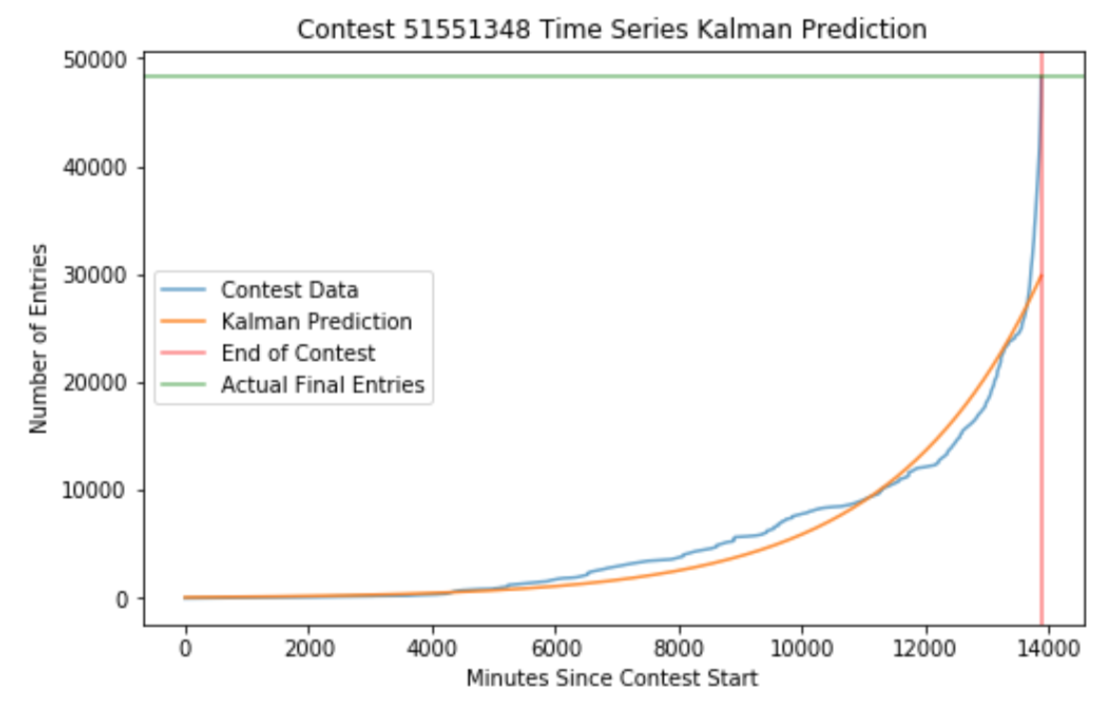
\includegraphics[width=8cm]{body/methodology/KF_True0.png}
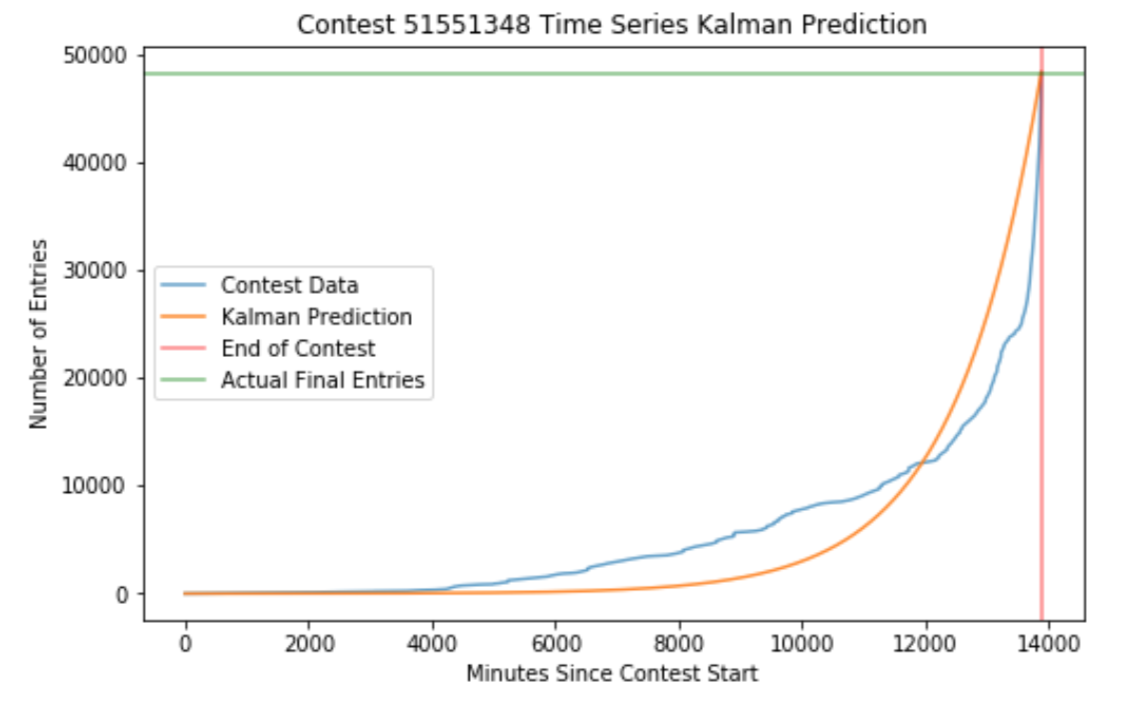
\includegraphics[width=8cm]{body/methodology/KF_True10.png}
\caption{Temp EKF Q=0/ EKF Q=10}
\end{figure}